% Aumentar a introdução antes da notação formal do problema

\documentclass[runningheads,a4paper]{llncs}

\usepackage{amssymb}
% ADD THOSE LIBS AT THE PACKAGE FOR THE JOURNAL
\usepackage{mathtools}
\usepackage{verbatim}

\setcounter{tocdepth}{3}
\usepackage{graphicx}

% ADD THOSE LIBS AT THE PACKAGE FOR THE JOURNAL
\usepackage{algorithm}
\usepackage{algpseudocode}

\usepackage{url}
\urldef{\mail}\path|{hbecker, buriol}@inf.ufrgs.br|
\newcommand{\keywords}[1]{\par\addvspace\baselineskip
\noindent\keywordname\enspace\ignorespaces#1}

\begin{document}

\mainmatter  % start of an individual contribution

% first the title is needed
\title{UKP5: a New Algorithm for the Unbounded Knapsack Problem}

% a short form should be given in case it is too long for the running head
\titlerunning{UKP5: a new algorithm for the UKP}

\author{Henrique Becker \and Luciana S. Buriol}
% (feature abused for this document to repeat the title also on left hand pages)
\authorrunning{UKP5: a new algorithm for the UKP}

\institute{Federal University of Rio Grande do Sul (UFRGS),\\
Porto Alegre, Brazil\\
\mail\\
\url{http://ppgc.inf.ufrgs.br/}
}

%\toctitle{Lecture Notes in Computer Science}
%\tocauthor{Authors' Instructions}
\maketitle

\begin{abstract}
In this paper we present UKP5, a novel algorithm for solving the unbounded knapsack problem. 
UKP5 is based on dynamic programming, but implemented in a non traditional way: instead of looking backward for stored values of subproblems, 
it stores incremental lower bounds forward. 
UKP5 uses sparsity, periodicity, and dominance for speeding up computation. 
UKP5 is considerably simpler than EDUK2, the state-of-the-art algorithm for solving the problem. 
Moreover, it can be naturally implemented using the imperative paradigm, differently from EDUK2. 
We run UKP5 and EDUK2 on a benchmark of hard instances proposed by the authors of EDUK2. 
The benchmark is composed by 4540 instances, divided into five classes, with instances ranging from small to large inside each class. 
Speedups were calculated for each class, and the overall speedup was calculated as the classes speedups average. 
The experimental results reveal that UKP5 outperforms EDUK2, being 47 times faster on the overall average.
\keywords{unbounded knapsack problem, dynamic programming, combinatorial optimization}
\end{abstract}

\section{Introduction}

The unbounded knapsack problem (UKP) is a variation of the well-known bounded knapsack problem (BKP).
UKP allows the allocation of an unbounded quantity of each item type.

The UKP is NP-Hard, and thus has no known polynomial-time algorithm for solving it. 
However, it can be solved by a pseudo-polynomial dynamic programming algorithm.
UKP arises in real world problems mainly as a subproblem of the Bin Packing Problem (BPP) and Cutting Stock Problem (CSP). 
Both BPP and CSP are of great importance for the industry \cite{survey2014}\cite{gg-1}\cite{gg-2}. 
The currently fastest known solver for BPP/CSP\cite{survey2014}\cite{belov} 
uses a technique (introduced in \cite{gg-1}) that needs to solve an UKP instance as the pricing problem at each iteration of a column generation approach. 
The need for efficient algorithms for solving the UKP is fundamental for the overall performance of the column generation.

Two techniques are often used for solving UKP: dynamic programming (DP) \cite[p. 214]{gar72}\cite{eduk}\cite[p. 311]{tchu} and branch and bound (B\&B) \cite{mtu2}. 
The DP approach has a stable pseudo-polynomial time algorithm linear on the capacity and number of items. 
The B\&B approach can be less stable. 
It can be faster than DP on instances with some characteristics, such as when the remainder of the division between the weight of the best item by capacity is small; or the items have a big efficiency variance. Nonetheless, B\&B has always the risk of an exponential time worst case.

The state-of-the-art solver for the UKP, introduced by~\cite{pya}, is a hybrid solver that combines DP and B\&B. 
It tries to solve the problem by B\&B, and if this fails to solve the problem quickly, it switches to DP using some data gathered by the B\&B to speed up the process. 
The solver's name is PYAsUKP, and it is an implementation of the EDUK2 algorithm.%We have found that the DP used by PYAsUKP is very slow when compared to our algorithm. Even solving some instances in less than a centisecond using B\&B, the solver is yet about thirty times slower than our method, in average. Also, our algorithm is much less complex, and can be easily implemented on a imperative language. The periodicity stop condition, and the solution dominance concept, used on UKP55 are algorithm specific. So we don't count them as individual contributions.

%The recent paper \cite{parallellUKP} proposes, implements and compares two parallelization approaches for classical DP formulations of the UKP. 
%It doesn't compare with the state-of-the-art but, regarding to PYAsUKP, states that ``The algorithm (PYAsUKP) significantly outperforms all existing algorithms for solving the problem.''.

% \footnote{The order of the items doesn't change the optimal solution value. Nonetheless, the order of the items is relevant for some algorithms performance, and we will refer to items by its position in the item list. For these reasons we will refer to the input items as a list, and not as a set.}

\subsection{UKP Formal Notation}

The following notation of the UKP will be used for the rest of the paper. An UKP instance is composed by a capacity \(c\), and a list of \(n\) items.
Each item can be referenced by its index in the item list \(i \in \{1\dots n\}\). 
Each item \(i\) has a weight value \(w_i\), and a profit value \(p_i\).
A solution is an item multiset, i.e, a set that allows multiple copies of the same element.
The sum of the items weight, or profit, of a solution \(s\) is denoted by \(w_s\), or \(p_s\).
A valid solution \(s\) has \(w_s \leq c\).
An optimal solution \(s*\) is a valid solution with the greatest profit among all valid solutions.
%We refer to the profit value shared among all optimal solutions for a capacity \(y\) as \(opt(y)\), if we omit the capacity then \(c\) is implied; 
The UKP objective is to find an optimal solution for the given UKP instance. 
The mathematical formulation of UKP is:

\begin{align}
  maximize: &\sum_{i=1}^n p_i x_i\label{eq:objfun}\\
subject~to: &\sum_{i=1}^n w_i x_i \leq c\label{eq:capcons}\\
            &x_i \in \mathbb{N}_0\label{eq:x_integer}
\end{align}

%\footnote{If the quantities weren't restricted to the integers the problem wouldn't be NP-Hard.}
The quantities of each item \(i\) in an optimal solution are denoted by \(x_i\), and are restricted to the non-negative integers, as~\eqref{eq:x_integer} indicates. 
We assume that the capacity \(c\), the quantity of items \(n\) and the weights of the items \(w_i\) are positive integers. 
The profits of the items \(p_i\) are positive real numbers.

%\footnote{If the efficiencies tie the best item is the item with the lowest weight between the tied items.}
The efficiency of an item \(i\) is the ratio \(\frac{p_i}{w_i}\), and is denoted by \(e_i\). 
We use \(w_{min}\) and \(w_{max}\) to denote the smallest item weight, and the biggest item weight, respectively. 
Also, we refer to the item with the lowest weight among the ones with the greatest efficiency as the \emph{best item}, 
and the item with the lowest weight among all items as the \emph{smallest item}.
If two or more items have the same weight we consider only the one with the best profit (the others can be discarded without loss to the optimal solution value), if they have the same weight and profit we consider them the same item.

% AlgorithmsForKnapsackProblemsPsinger -- p. 148, cita 53 (Martello and Toth) to explain why do not transform unbounded knapsack instances in bounded (we could simply say that the lack of restrictions gives more opportunity for optimization) AND 
% Garfinkel, PYAsUKP

\subsection{Dominance}

Dominance, in the UKP context, is a technique for discarding items without affecting the optimal solution value. 
By this definition, every item that isn't used in an optimal solution could be discarded, but this would need the knowledge of the solution beforehand. 
Some dominances can be verified in polynomial time over \(n\), and can speed up the resolution of an NP-Hard problem reducing the instance input size. 
%, and allow to exclude items without affecting the optimal solution value. 
%It's easy to see that any polynomial-time algorithm that can be used to reduce the input of an exponential time algorithm is promising. 
Instances where many items can be excluded by the two simplest dominances (simple dominance and multiple dominance) are known as ``easy'' instances. 
Research on these two dominances was done to a large extent, leading to the following statement by Pisinger in 1995
%after enumerating the research done until the moment on UKP 
``[...] perhaps too much effort has been previously been used on the solution of easy data instances.'' \cite[p. 20]{pisinger1995}.

Other two important dominances are collective dominance and threshold dominance \cite{pya}. 
These two dominances are too time demanding to be applied at a preprocessing phase, differently from simple and multiple dominance. 
They are often integrated in the UKP algorithm, and remove items while the algorithm executes. 
The collective dominance needs to know the \(opt(y)\) to exclude an item \(i\) with \(w_i = y\), where \(opt(y)\) is the optimal solution value for a capacity $y$.
The threshold dominance needs to know the \(opt(\alpha\times w_i)\) to exclude the item \(i\) from capacity \(y = \alpha\times w_i\) onwards, where \(\alpha\) is any positive integer.

%The specifics of these four dominances are very well described at \cite{pya}. 
%The UKP5 doesn't make use of any of those four dominances. 
%It uses a ``solution dominance'' approach that is implicit in the algorithm and achieves results similar to the four dominances. The decision to not use the known dominances is based on two main points: UKP5 was made to solve hard data instances, applying the dominance over hard data instances don't always pay off; our ``solution dominance'' already excludes items, so any benefits of the dominances would be diminished, but the cost would be the same. 
%For the rest of the article, when we say that an specific item is dominated, we are saying that it could be excluded without changing \(opt\).

%UKP5 uses a single test that cover the four dominances. We call this approach ``solution dominance''.

% CITE ``'' p. 20, Pisinger

% In \cite{\cite{CPISINGER}}, a complete analysis of the simplest dominance type (simple/multiple dominance) is given. 

\subsection{Periodicity}

A periodicity bound \(y^{*}\) is an upper capacity bound for the existence of optimal solutions without the best item. 
In another words, it's a guarantee that any solution for an instance where \(y^{*} \leq c\) has at least one copy of the best item. 
The periodicity bound is specially useful because it can be applied repeatedly. 
For example, let \(c = 1000\), \(y^{*} = 800\) and \(w_b = 25\) where \(b\) is the best item; because of \(y^{*} \leq c\) we know that any optimal solution has a copy of \(b\), so we can add one \(b\) to the solution and combine with an optimal solution for \(c = 975\); but \(975\) is yet bigger than \(800\), so we can repeat the process until \(c = 775\). 
This way, for any \(y^{*} \leq c\) we can reduce the UKP instance capacity by \(max(1, \lceil(c-y^{*})/w_b\rceil)\times w_b\) and add to a reduced instance optimal solution \(max(1, \lceil(c-y^{*})/w_b\rceil)\) copies of \(b\).

There exist many proposed periodicity bounds, but some are time consuming (as \(O(n^2)\)\cite{badbound1}), others depend on specific instance characteristics (as \cite{badbound2}\cite{pya}).
We used only a UKP5-specific periodicity bound described later and the \(y^{*}\) bound described in~\cite[p. 223]{gar72}.
The $y^*$ is \(O(1)\) on an item list ordered by non-increasing efficiency,  and it is generic, being successfuly applied on instances of most classes.
Assuming $i$ is the best item, and $j$ is the second most efficient item, then \mbox{\(y^{*} = p_i / (e_i - e_j)\)}.




\subsection{Sparsity}

% Any weight difference between one solution and the next distinct solution can't be bigger than \(w_{min}\).
%The classic DP algorithm for UKP would compute the optimal solution value for every capacity and use them later to compute the optimal solution value for bigger capacities. This approach can become inefficient when the \(w_{min}\) becomes big. Lets suppose that we have an array of \(c\) positions, each with an optimal solution for that capacity value. As there can be many optimal solutions for the same capacity, we will use always the one with the lowest weight. If \(w_{min}\) is small, for example \(w_{min} = 1\), then we have the guarantee that every capacity has a distinct optimal solution. Otherwise, if \(w_{min}\) is big, for example \(w_{min} = 10^4\), it's possible to have ranges of hundreds or thousands of capacities with the same optimal solution. The classical DP algorithm would iterate this range and execute \(O(n)\) operations at each capacity, resulting in an optimal solution with the same profit value at each capacity. 

For some UKP instances, not every non-zero capacity value can be obtained by a linear combination of the items weight. 
If \(w_{min}\) is small, for example \(w_{min} = 1\), we have the guarantee that every non-zero capacity has at least one solution with weight equal to the capacity value.
But if \(w_{min}\) is big, for example \(w_{min} = 10^4\), there can be a large number of capacities with no solution comprising weight equal to the capacity. 
These capacities have an optimal solution that don't fill the capacity completely. 
The UKP5 exploits sparsity in the sense that it avoids computing the optimal solution value for those unfulfilled capacities. 
%When the algorithm ends, it searches the range where the optimal solution value for \(c\) is guaranteed to be. 
The array that stores the optimal solutions value is, therefore, sparse.

\section{UKP5: The Proposed Algorithm}
\label{sec:ukp5}

UKP5 is inspired by the DP algorithm described by Garfinkel~\cite[p. 221]{gar72}. 
The name ``UKP5'' is due to five improvements applied over that algorithm:

\begin{enumerate}
  \item Symmetry pruning: symmetric solutions are pruned in a more efficient fashion than in~\cite{gar72};
  \item Sparsity: not every position of the optimal solutions value array has to be computed;
  \item Dominated solutions pruning: dominated solutions are pruned;
  \item Time/memory tradeoff: the test \(w_i \leq y\) from the algorithm in~~\cite{gar72} was removed in cost of more O($w_{max}$) memory;
  \item Periodicity: the periodicity check suggested in~\cite{gar72} (but not implemented there) was adapted and implemented.
\end{enumerate}

\begin{algorithm}[!t]
\caption{UKP5 -- Computation of $opt$}\label{alg:ukp5}
\begin{algorithmic}[1]
\Procedure{UKP5}{$n, c, w, p, w_{min}, w_{max}$}
  \State \(g \gets\) array of \(c + w_{max}\) positions each one initialized with \(0\)\label{create_g}
  \State \(d \gets\) array of \(c + w_{max}\) positions each one initialized with \(n\)\label{create_d}
  
  \For{\(i \gets 1, n\)}\label{begin_trivial_bounds}\Comment{Stores one-item solutions}
    \If{\(g[w_i] < p_i\)}
      \State \(g[w_i] \gets p_i\)
      \State \(d[w_i] \gets i\)
    \EndIf
  \EndFor\label{end_trivial_bounds}

  \State \(opt \gets 0\)\label{init_opt}

  \For{\(y \gets w_{min}, c\)}\label{main_ext_loop_begin}\Comment{Can end early because of periodicity check}
    \If{\(g[y] \leq opt\)}\label{if_less_than_opt_begin}\Comment{Handles sparsity and pruning of dominated solutions}
    	\State \textbf{continue}\label{alg:continue}\Comment{Ends current iteration and begins the next}
    \EndIf\label{if_less_than_opt_end}
    
    \State \(opt \gets g[y]\)\label{update_opt}
    
    \For{\(i=1,d[y]\)}\label{main_inner_loop_begin}\Comment{Creates new solutions (never symmetric)}
      \If{\(g[y + w_i] < g[y] + p_i\)}\label{if_new_lower_bound_begin}
        \State \(g[y + w_i] \gets g[y] + p_i\)
        \State \(d[y + w_i] \gets i\)
%      \ElsIf{\(g[y + w_i] = g[y] + p_i \land i < d[y + w_i]\)}
%        \State \(d[y + w_i] \gets i\)
      \EndIf\label{if_new_lower_bound_end}
    \EndFor\label{main_inner_loop_end}
  \EndFor\label{main_ext_loop_end}
  \State \textbf{return} \(opt\)

%  \For{\(y \gets c-w_{min}+1, c\)}\label{get_y_opt_loop_begin}\Comment{Removal of dominated solutions}
%    \If{\(g[y] > opt\)}\label{last_loop_inner_if}
%      \State \(opt \gets g[y]\)
%      \State \(y_{opt} \gets y\)
%    \EndIf
%  \EndFor\label{get_y_opt_loop_end}
\EndProcedure
\end{algorithmic}
\end{algorithm}

A pseudocode of our algorithm is presented in Algorithm~\ref{alg:ukp5}.
We have two main data structures, the arrays \(g\) and \(d\), both with dimension $c - w_{min} + w_{max} + 1$. 
The \(g\) is a sparse array where we store solutions profit. If \(g[y] > 0\) then there exists a non-empty solution \(s\) with \(w_s = y\) and \(p_s = g[y]\). 
The \(d\) array stores the index of the last item used on a solution. If \(g[y] > 0 \land d[y] = i\) then the solution \(s\) with \(w_s = y\) and \(p_s = g[y]\) has at least one copy of item \(i\). 
This array makes trivial to recover the optimal solution, but its main use is to prune solution symmetry.

Our first loop (lines \ref{begin_trivial_bounds} to \ref{end_trivial_bounds}) simply stores all solutions made of a single item in the arrays \(g\) and \(d\). 
For a moment, let's ignore lines \ref{if_less_than_opt_begin} to \ref{if_less_than_opt_end}, and replace \(d[y]\) at line \ref{main_inner_loop_begin} by \(n\). 
With these changes, the second loop (between lines \ref{main_ext_loop_begin} and \ref{main_ext_loop_end}) 
iterates \(g\) and when it finds a stored solution (\(g[y] > 0\)) it tests \(n\) new solutions 
(the combinations of the current solution with every item). 
Then, it replaces solutions already stored if exists a new solution with the same weight and a greater profit.

When we add the lines \ref{if_less_than_opt_begin} to \ref{if_less_than_opt_end} to the algorithm, it stops creating new solutions from dominated solutions. 
%We use the \textbf{continue} keyword at line \ref{alg:continue} meaning the current iteration ends, and the next iteration begins (as is common in C-like programming languages). 
If a solution \(s\) with a smaller weight (\(w_s < y\)) has a bigger profit (\(p_s = opt > p_t\), where \(w_t = y \land p_t = g[y]\)), then \(s\) dominates \(t\). 
If solution \(s\) dominates \(t\) then, for any item \(i\), the \(s \cap \{i\}\) solution will dominate the \(t \cap \{i\}\) solution. 
This way, new solutions created from \(t\) are guaranteed to be dominated by the solutions created from \(s\). 
A whole superset of \(t\) can be discarded without loss to solution optimality. 

The change from \(n\) to \(d[y]\) is based on the algorithm from~\cite{gar72} and it prunes symmetric solutions.
In a naive DP algorithm, if the item multiset \(\{5, 3, 2\}\) is a valid solution, then every permutation of it is reached in different ways, wasting processing time. 
To avoid computing symmetric solutions, we enforce non-increasing order of the items index. 
Any item inserted on a solution \(s\) has an index that is equal to or lower than the index of the last item inserted on \(s\). 
This way, solution \(\{2,3,5,10\}\) cannot be reached.
However, this is not a problem because this solution is equal to \(\{10, 5, 3, 2\}\), and this solution can be reached. 
%No solution stops being generated, but they will always be generated from the greatest item index to the lowest item index.
%\footnote{The algorithm would compute \(\{1, 2, 3\} \cap \{1\}\) and \(\{1, 1, 2\} \cap \{3\}\), for example.}

When the two changes are combined, and the items are sorted by non-increasing efficiency, UKP5 gains in performance. 
The UKP5 iterates by the item list only when it finds a non-dominated solution, i.e, $g[y] \geq 0$ (line \ref{if_less_than_opt_begin}). 
Non-dominated solutions are more efficient (larger ratio of profit by weight) than the skipped dominated solutions. 
%Efficient solutions are efficient because are composed by efficient items. 
%When sorted by non-increasing efficiency, efficient items have the lowest index values. 
Therefore, the UKP5 inner loop (lines \ref{main_inner_loop_begin} to \ref{main_inner_loop_end}) often iterates up to a low \(d[y]\) value. 
Experimental results show that, after some threshold capacity, the UKP5 inner loop consistently iterates only for a small fraction of the item list.
%The threshold capacity depends on the value of \(w_{max}\).
%, sometimes only the 2\% most efficient items, for the remaining capacities.

%Provar que o algoritmo encontra a solução ótima com o menor peso, além de ser a de maior profit.
%The third loop (lines \ref{get_y_opt_loop_begin} to \ref{get_y_opt_loop_end}) gets the optimal solution value, and the corresponding optimal solution weight. 
%Any optimal solution %not excluded by our solution dominance test (\ref{if_less_than_opt_begin} to \ref{if_less_than_opt_end}), 
%is guaranteed to have weight between \(c - w_{min} + 1\) and \(c\) (both inclusive). 
%The proof is simple. A valid solution can't weight more than \(c\), and for any solution \(s\) that weights less than \(c - w_{min} + 1\), we can obtain a solution with a bigger profit inserting a copy of \(i\) to \(s\), where \(w_i = w_{min}\). When the algorithm ends, the \(opt\) variable holds the optimal solution value, and \(y_{opt}\) holds the the corresponding weight. 

The algorithm ends with the optimal solution stored at \(opt\). The solution assemble phase isn't described in algorithm \ref{alg:ukp5}. 
But it's similar to the one used by the DP method described in \cite[p. 221, Steps 6-8]{gar72}. 
Let \(y_{opt}\) be a capacity where \(g[y_{opt}] = opt\). We add a copy of item \(i = d[y_{opt}]\) to the solution, then we add a copy of item \(j = d[y_{opt} - w_i]\), and so on, until \(d[0]\) is reached. 
This phase has a \(O(c)\) time complexity, as the solution can be composed of \(c\) copies of an item \(i\) with \(w_i = 1\).

% ADICIONAR PARÁGRAFO SOBRE FASE DE MONTAR A SOLUÇÃO

\subsection{Solution Dominance}

%\footnote{Note that, on ukp5, the lowest index of an item in a solution is also the index of the last item inserted in the solution (and consequently the value stored at \(d[y]\) where \(y\) is the solution weight).}
In this section we discuss how the solution dominance speeds up UKP5. 
The solution dominance happens because of the test in lines \ref{if_less_than_opt_begin} to \ref{if_less_than_opt_end}, the use of \(d[y]\) in line \ref{main_inner_loop_begin}, and is affected by the item list order (happens more often if the item list is sorted by non-increasing efficiency). 
We use the \(min_{ix}(s)\) notation to refer to the lowest index between the items that compose the solution \(s\). The \(max_{ix}(s)\) notation has analogue meaning.

When a solution \(t\) is pruned because \(s\) dominates \(t\) (lines \ref{if_less_than_opt_begin} to \ref{if_less_than_opt_end}), some solutions \(u\), where \(u \supsetneq t\), are not generated. 
If \(s\) dominates \(t\) and \(u \supsetneq t \land max_{ix}(u\setminus t) \leq min_{ix}(t)\) then \(u\) is not generated by UKP5. 
In other words, if \(\{3, 2\}\) is dominated, then \(\{3, 2, 2\}\) and \(\{3, 2, 1\}\) are not be generated by UKP5. 
This is true only for solutions \(\{3, 2\} \cap v\), where \(v\) has only indexes lower than or equal to \(2\). 
Ideally, any \(u\) where \(u \supsetneq t\) should not be generated as it will be dominated by a solution \(x\) where \(x \supsetneq s\) anyway. 
It's interesting to note that this happens eventually, as any \(t \cap \{i\}\) where \(i > min_{ix}(t)\) will be dominated by \(s \cap \{i\}\) (or by a solution that dominates \(s \cap \{i\}\)), and at some point no solution that is a superset of \(t\) is generated.

%We would like to point again that a dominated solution and its supersets can always be excluded from the problem without affecting the optimal solution value. 
%A dominated solution always have a dominant solution, and the dominant solution have the same or more profit value, and the same or less weight. This way, the dominant solution can always be used in place of the dominated one without loss to the optimal solution value. 

\subsection{Implementation details}

With the purpose of making the initial explanation simpler, we have omitted some steps that are relevant to the algorithm performance, but not essential for accessing its correctness. 
A complete overview of the omitted steps is presented at this section.

% A QUESTÃO DO NÃO USO DAS DOMINANCIAS JÁ È DITA ANTES, REMOVER AQUI?
All the items are sorted by non-increasing efficiency and, between items with the same efficiency, by increasing weight. 
This speed ups the algorithm, but does not affect its correctness.
%The simple/multiple, collective or threshold dominances aren't used by UKP5, as this is often counterproductive for hard instances, where the undominated-to-all-items ratio is close to one, and superseded by our implicit solution dominance. 

The \(y^{*}\) periodicity bound is computed as in~\cite[p. 223]{gar72}, and used to reduce the \(c\) value. 
We further proposed an UKP5-specific periodicity check that was successfully applied. 
This periodicity check isn't used to reduce the \(c\) capacity before starting UKP5, as \(y^{*}\). 
The periodicity check is a stopping condition inside UKP5 main loop (\ref{main_ext_loop_begin} and \ref{main_ext_loop_end}). 
Let \(y\) be the value of the variable \(y\) at line \ref{main_ext_loop_begin}, and let \(y'\) be the biggest capacity where \(g[y'] \neq 0 \land d[y'] > 1\). 
If at some moment \(y > y'\) then we can stop the computation and fill the remaining capacity with copies of the first item (item of index \(1\)).
This periodicity check works only if the first item is the best item. 
If this assumption is false, then the described condition will never happen, and the algorithm will iterate until \(y = c - w_{min}\) as usual. The correctness isn't affected.

There's an \emph{else if} test at line \ref{if_new_lower_bound_end}. 
If \(g[y + w_i] = g[y] + p_i \land i < d[y + w_i]\) then \(d[y] \gets i\). 
This may seem unnecessary, as appears to be an optimization of a rare case, where two solutions have the same weight and profit. 
Nonetheless, without this test, the UKP5 was about 1800 (one thousand and eight hundreds) times slower on some subset-sum instance datasets.
%presented at Table~\ref{tab:times}.
%For other instance classes, no significant speedup was observed.

We iterate only until \(c-w_{min}\) (instead of \(c\), in line \ref{main_ext_loop_begin}), as it is the last \(y\) value that can affect \(g[c]\)). After this we search for a value greater than \(opt\) in the range \(g[c-w_{min}+1]\) to \(g[c]\) and update \(opt\).

\section{Computational Results}
% Describe all instance datasets.
% Describe the environment (computer, isolated cores, disabled hyperthreading)
% Only used internal time, internal time of PYAsUKP was strange
% external time not used because HD data reading race conditions, and different reading methods
% TABLE WITH RESULTS
In this section we describe the experiments environment, instance sets and results. We compare our UKP5 implementation, and the EDUK2 implementation provided by~\cite{pya} (called PYAsUKP). 
The used source codes can be found at \url{https://github.com/henriquebecker91/masters/tree/v0.1}\footnote{The UKP5 implementation is at \textbf{codes/cpp/} and two versions of PYAsUKP are at \textbf{codes/ocaml/}. The \emph{pyasukp\_site.tgz} is the version used to generate the instances, and was also available at \url{http://download.gna.org/pyasukp/pyasukpsrc.html}. 
A more stable version was provided by the authors. 
This version is in \emph{pyasukp\_mail.tgz} and it was used to solve the instances the results presented in Table~\ref{tab:times}. 
The \emph{create\_*\_instances.sh} scripts inside \textbf{codes/sh/} were used to generate the instance datasets.}. 
The times reported were given by the tools themselves and do not count the instance loading time. 
The runs external time\footnote{Given by the \textit{time} application, available at \url{https://www.archlinux.org/packages/extra/x86_64/time/}. 
The bash internal command was \emph{not} used.} were also captured and no significant discrepancy was observed. 
Therefore, we have chosen to use the times reported by PYAsUKP and UKP5 (as is the common practice). 
For all instances, the weight, profit and capacity are integral.

We use the following notation: \(rand(x, y)\) means a random integer between \(x\) and \(y\) (both inclusive); \(x\overline{n}\) means \(x\) as a string concatenated with the value of variable \(n\) as a string. For example: if \(n = 5000\) then \(10\overline{n} = 105000\).

%We could not determine if the methods used by PYAsUKP to generate random integer sets results in an uniform distribution. We advice checking the source code for more information on the exact method used for obtaining random integer sets.

\subsection{Environment}

The computer used on the experiments was an ASUS R552JK-CN159H. The CPU has four physical cores (Intel Core i7-4700HQ Processor, 6M Cache, 3.40 GHz). 
The operating system used was Linux nymeria 4.3.3-2-ARCH x86\_64 GNU/Linux (i.e. Arch linux). 
Three of the four cores were isolated using the \emph{isolcpus} kernel flag. 
The \emph{taskset} utility was used to execute UKP5 and PYAsUKP in parallel on the isolated cores. 
The computer memory was never completely used (no swapping was done). 
The UKP5 code was compiled with gcc (g++) version 5.3.0 (the \emph{-O3 -std=c++11} flags were enabled).

\subsection{Instance Sets}

The instance sets aim to reproduce the ones described in~\cite{pya}. 
The same tool was used to generate the datasets (PYAsUKP), and the same parameters were used, otherwise noted the contrary. 
In Subsection 5.1.1 \emph{Known ``hard'' instances} of~\cite{pya} some sets of easy instances are used to allow comparison with MTU2. 
However, the authors reported integer overflow problems with  MTU2 on harder instances. 
With exception of the subset-sum dataset, all datasets have a similar harder set (Subsection 5.2.1 \emph{New hard UKP instances}~\cite{pya}).
Thus, we considered in the runs only the harder ones. 
Each instance has a random capacity value within intervals shown in Table~\ref{tab:times}. 
The PYAsUKP parameters \mbox{\emph{-wmin \(w_{min}\) -cap c -n \textbf{n}}} were used in all instances generation. 
%When we found a discrepancy between the formula presented in \cite{pya} and the PYAsUKP code, or generated instances, we opted for changing the formula based on the observed behavior. 
%As our knowledge of OCaml is limited, we cannot guarantee that the formula presented here is a perfect match for the code; but, based by the generated instances, we believe it to be correct to a good extent.
We found some small discrepancies between the formulas presented in~\cite{pya} and the ones used in PYAsUKP code.
We opted for using the ones from  PYAsUKP code, and they are presented below.

\subsubsection{Subset-Sum}\label{sec:subsetsum}
Instances generated with \(p_i = w_i = rand(w_{min}, w_{max})\). 
The majority of the subset-sum instances used in \cite{pya} were solved on less than a centisecond in our experiments. 
This makes easy to have imprecise measuring. 
Because of this, in this paper, we use a similar dataset, but with each parameter multiplied by ten. 
Therefore, we generated 10 instances for each possible combination of: \(w_{min} \in \{10^3, 5\times10^3, 10^4, 5\times10^4, 10^5\}\); \(w_{max} \in \{5\times10^5, 10^6\}\) and \(n \in \{10^3, 2\times10^3, 5\times10^3, 10^4\}\), totaling 400 instances. We do not discriminate each combination in~Table \ref{tab:times} for brevity. The PYAsUKP \emph{-form ss -wmax \(w_{max}\)} parameters were used.

\subsubsection{Strong Correlation}
Instances generated using the following formula: \(w_i = w_{min} + i - 1\) and \(p_i = w_i + \alpha\), for a given \(w_{min}\) and \(\alpha\).  Note that, except by the random capacity, all instances with the same \(\alpha\), \(\mathbf{n}\) and \(w_{min}\) combination are equal. The formula don't rely on random numbers. The PYAsUKP \emph{-form chung -step \(\alpha\) } parameters were used.

\subsubsection{Postponed Periodicity}
This family of instances is generated by the following method: \textbf{n} distinct weights are generated with \(rand(w_{min}, w_{max})\) and then sorted by increasing order; \(p_1 = w_1 + rand(1, 500)\); and \(\forall i \in [2, n].~p_i = p_{i-1} + rand(1, 125)\). The PYAsUKP \emph{-form nsds2 -step 500 -wmax \(w_{max}\)} parameters were used.

\subsubsection{No Collective Dominance}
This family of instances is generated by the following method: \textbf{n} distinct weights are generated with \(rand(w_{min}, w_{max})\) and then sorted by increasing order; \(p_1 = p_{min} + rand(0, 49)\); and \(\forall i \in [2, n].~p_i = \lfloor w_i \times ((p_{i-1}/w_{i-1}) + 0.01)\rfloor + rand(1, 10)\). The given values are: \(w_{min} = p_{min} = \mathbf{n}\) and \(w_{max} = 10\overline{n}\). The PYAsUKP \emph{-form hi -pmin \(p_{min}\) -wmax \(w_{max}\)} parameters were used.

\subsubsection{SAW}
This family of instances is generated by the following method: generate \textbf{n} random weights between \(w_{min}\) and \(w_{max} = 1\overline{n}\) with the following property: \(\forall i \in [2, n].~w_i~mod~w_1 > 0\) (\(w_1\) is the smallest weight); sort by increasing order; then \(p_1 = w_1 + \alpha\) where \(\alpha = rand(1,5)\), and \(\forall i \in [2, n].~p_i = rand(l_i, u_i)\) where \(l_i = max(p_{i-1}, q_i)\), \(u_i = q_i + m_i\), \(q_i = p_1 \times \lfloor w_i / w_1 \rfloor \), and \(m_i = w_i~mod~w_1\). The PYAsUKP \emph{-form saw -step \(\alpha\) -wmax \(w_{max}\)} parameters were used.

\subsection{Results and Analysis}

Table \ref{tab:times} presents the times used by UKP5 and PYAsUKP to solve the instance classes previously described. No time limit was defined. Figure \ref{fig:times} presents the same data, in logarithmic scale.

\begin{table}
\caption{Columns \textbf{n} and \(w_{min}\) values must be multiplied by \(10^3\) to obtain their true value. Let \(T\) be the set of times reported by UKP5 or EDUK2, then the meaning of the columns \textbf{avg}, \textbf{sd}, \textbf{min} and \textbf{max}, is, respectively, the arithmetic mean of \(T\), the standard deviation of \(T\), the minimal value of \(T\) and the maximal value of \(T\). The time unit of the table values is seconds.}
\label{tab:times}
\def\arraystretch{1.1}
\setlength\tabcolsep{4px}

\begin{tabular}{@{\extracolsep{4pt}}rrrrrrrrrrr@{}}

\hline
\multicolumn{3}{l}{Instance desc.} & \multicolumn{4}{l}{UKP5} & \multicolumn{4}{l}{PYAsUKP}\\
\cline{1-3}\cline{4-7}\cline{8-11}

\multicolumn{3}{l}{400 inst. per line} & \multicolumn{8}{l}{Subset-sum. Random \emph{c} between \([5\times10^6; 10^7]\)}\\
\cline{1-3}\cline{4-11}

& \textbf{n} & \(w_{min}\)  & \textbf{avg} & \textbf{sd} & \textbf{min} & \textbf{max} & \textbf{avg} & \textbf{sd} & \textbf{min} & \textbf{max}\\
\cline{1-3}\cline{4-7}\cline{8-11}

\multicolumn{3}{c}{See section~\ref{sec:subsetsum}} & 0.08 & 0.20 & 0.01 & 1.42 & 6.39 & 55.33 & 0.00 & 726.34\\
\hline

\multicolumn{3}{l}{20 inst. per line} & \multicolumn{8}{l}{Strong correlation. Random \emph{c} between \([20\overline{n}; 100\overline{n}]\)}\\
\cline{1-3}\cline{4-11}
\textbf{\(\alpha\)} & \textbf{n} & \(w_{min}\) & \textbf{avg} & \textbf{sd} & \textbf{min} & \textbf{max} & \textbf{avg} & \textbf{sd} & \textbf{min} & \textbf{max}\\
\cline{1-3}\cline{4-7}\cline{8-11}
 5 & 5  & 10 & 0.05 & 0.00 & 0.05 & 0.05 & 2.46 & 2.81 & 0.00 & 6.13\\
   &    & 15 & 0.07 & 0.00 & 0.07 & 0.09 & 5.84 & 2.43 & 0.00 & 8.82\\
   &    & 50 & 0.20 & 0.06 & 0.08 & 0.24 & 18.35 & 12.64 & 0.00 & 50.58\\
 5 & 10 & 10 & 0.11 & 0.01 & 0.10 & 0.14 & 0.00 & 0.00 & 0.00 & 0.01\\
   &    & 50 & 0.49 & 0.03 & 0.47 & 0.60 & 41.97 & 33.97 & 0.00 & 93.18\\
   &    & 110 & 1.07 & 0.02 & 1.05 & 1.13 & 147.60 & 114.39 & 0.00 & 342.86\\
-5 & 5  & 10 & 0.06 & 0.00 & 0.06 & 0.07 & 5.98 & 4.02 & 0.00 & 11.99\\
   &    & 15 & 0.09 & 0.00 & 0.08 & 0.10 & 10.37 & 6.73 & 0.00 & 21.00\\
   &    & 50 & 0.21 & 0.05 & 0.09 & 0.24 & 39.31 & 30.16 & 0.00 & 89.44\\
-5 & 10 & 10 & 0.19 & 0.01 & 0.17 & 0.21 & 13.13 & 12.61 & 0.00 & 33.00\\
   &    & 50 & 0.54 & 0.02 & 0.52 & 0.59 & 82.97 & 71.22 & 0.00 & 206.74\\
   &    & 110& 1.08 & 0.02 & 1.07 & 1.13 & 261.61 & 246.21 & 0.00 & 721.89\\
\hline

\multicolumn{3}{l}{200 inst. per line} & \multicolumn{8}{l}{Postponed periodicity. Random \emph{c} between \([w_{max}; 2\times10^6]\)}\\
\cline{1-3}\cline{4-11}
& \textbf{n} & \(w_{min}\) & \textbf{avg} & \textbf{sd} & \textbf{min} & \textbf{max} & \textbf{avg} & \textbf{sd} & \textbf{min} & \textbf{max}\\
\cline{1-3}\cline{4-7}\cline{8-11}
& 20 & 20 & 1.42 & 0.31 & 0.55 & 2.77 & 17.00 & 17.05 & 0.01 & 63.96\\
& 50 & 20 & 10.20 & 1.28 & 7.91 & 14.98 & 208.61 & 210.72 & 0.03 & 828.89\\
& 20 & 50 & 1.59 & 0.32 & 0.96 & 2.99 & 27.68 & 22.79 & 0.02 & 100.96\\
& 50 & 50 & 6.86 & 1.23 & 4.46 & 11.78 & 233.58 & 187.91 & 2.65 & 682.95\\
\hline

\multicolumn{3}{l}{500 inst. per line} & \multicolumn{8}{l}{No collective dominance. Random \emph{c} between \([w_{max}; 1000\overline{n}]\)}\\
\cline{1-3}\cline{4-11}
& \textbf{n} & \(w_{min}\) & \textbf{avg} & \textbf{sd} & \textbf{min} & \textbf{max} & \textbf{avg} & \textbf{sd} & \textbf{min} & \textbf{max}\\
\cline{1-3}\cline{4-7}\cline{8-11}
&  5 & n & 0.05 & 0.01 & 0.03 & 0.10 & 0.78 & 0.59 & 0.00 & 2.66\\
& 10 & n & 0.49 & 0.15 & 0.21 & 1.10 & 3.38 & 2.80 & 0.00 & 12.31\\
& 20 & n & 0.99 & 0.19 & 0.63 & 2.02 & 13.08 & 12.80 & 0.01 & 62.12\\
& 50 & n & 4.69 & 1.22 & 3.51 & 13.18 & 119.18 & 131.22 & 0.04 & 667.42\\
\hline

\multicolumn{3}{l}{\emph{qtd} inst. per line} & \multicolumn{8}{l}{SAW. Random \emph{c} between \([w_{max}; 10\overline{n}]\)}\\
\cline{1-3}\cline{4-11}
\textbf{qtd} & \textbf{n} & \(w_{min}\) & \textbf{avg} & \textbf{sd} & \textbf{min} & \textbf{max} & \textbf{avg} & \textbf{sd} & \textbf{min} & \textbf{max}\\
\cline{1-3}\cline{4-7}\cline{8-11}
~200 &  10 & 10 & 0.11 & 0.01 & 0.10 & 0.16 & 1.88 & 1.24 & 0.01 & 4.73\\
~500 &  50 &  5 & 0.74 & 0.08 & 0.66 & 1.98 & 4.79 & 4.22 & 0.02 & 17.78\\
~200 &  50 & 10 & 1.01 & 0.03 & 0.97 & 1.27 & 10.44 & 9.02 & 0.03 & 38.69\\
~200 & 100 & 10 & 14.13 & 2.96 & 9.95 & 21.94 & 60.58 & 54.08 & 0.05 & 192.04\\
\hline

\end{tabular}
\end{table}
Based on Table~\ref{tab:times}, except by one instance set that we will talk about later, we can make two statements: 1) the average time, standard deviation, and maximal time of UKP5 are always smaller than the PYAsUKP ones; 2) the minimal PYAsUKP time is always smaller than the UKP5 one.

Let's begin with the second statement. As EDUK2 uses a branch-and-bound (B\&B) algorithm before resorting to dynamic programming (DP), this is an expected result. 
Instances with big capacities and solutions that are composed by a large quantity of the best item, and a few non-best most efficient items, can be quickly solved by B\&B.
Our exception dataset (Strong Correlation, \(\alpha = 5\), \(n = 10\) and \(w_{min} = 10\)) is exactly this case. As said before, the strong correlation formula does not make use of random numbers, so all twenty instances of that dataset have the same items. 
The only thing that changes is the capacity. All solutions of this dataset are composed by hundreds of copies of the best item (that is also the smallest item, making the dataset even easier) and exactly one non-best item for making better use of the residual capacity (\(c~mod~w_1\)). 
All other datasets have instances that present the same characteristics, and because of that, the PYAsUKP minimal time is always close to zero. In Figure~\ref{fig:times} is possible to observe that there are many instances solved in less than 10 seconds by PYAsUKP which took longer for UKP5 to solve.
The number of instances where PYAsUKP was faster than UKP5 by instance class are: Subset-sum: 264 (\(\approx65\%\)); Strong correlation: 60 (\(25\%\)); Postponed periodicity: 105 (\(\approx13\%\)); No collective dominance: 259 (\(\approx13\%\)); SAW: 219 (\(\approx20\%\)). This from a total of 4540 instances.
%\footnote{The observant reader will see that, on the dataset ``Postponed periodicity'', \(n = 50\), \(w_{min} = 50\), PYAsUKP has a anomalous minimal time. On this dataset, the solution of the easiest instance is composed only by two items, the best one, and the 5317 most efficient one.}

% Put the importance of solving hard instances as they can have exponential time

\begin{figure}[th]
  \label{fig:times}
  \centering
  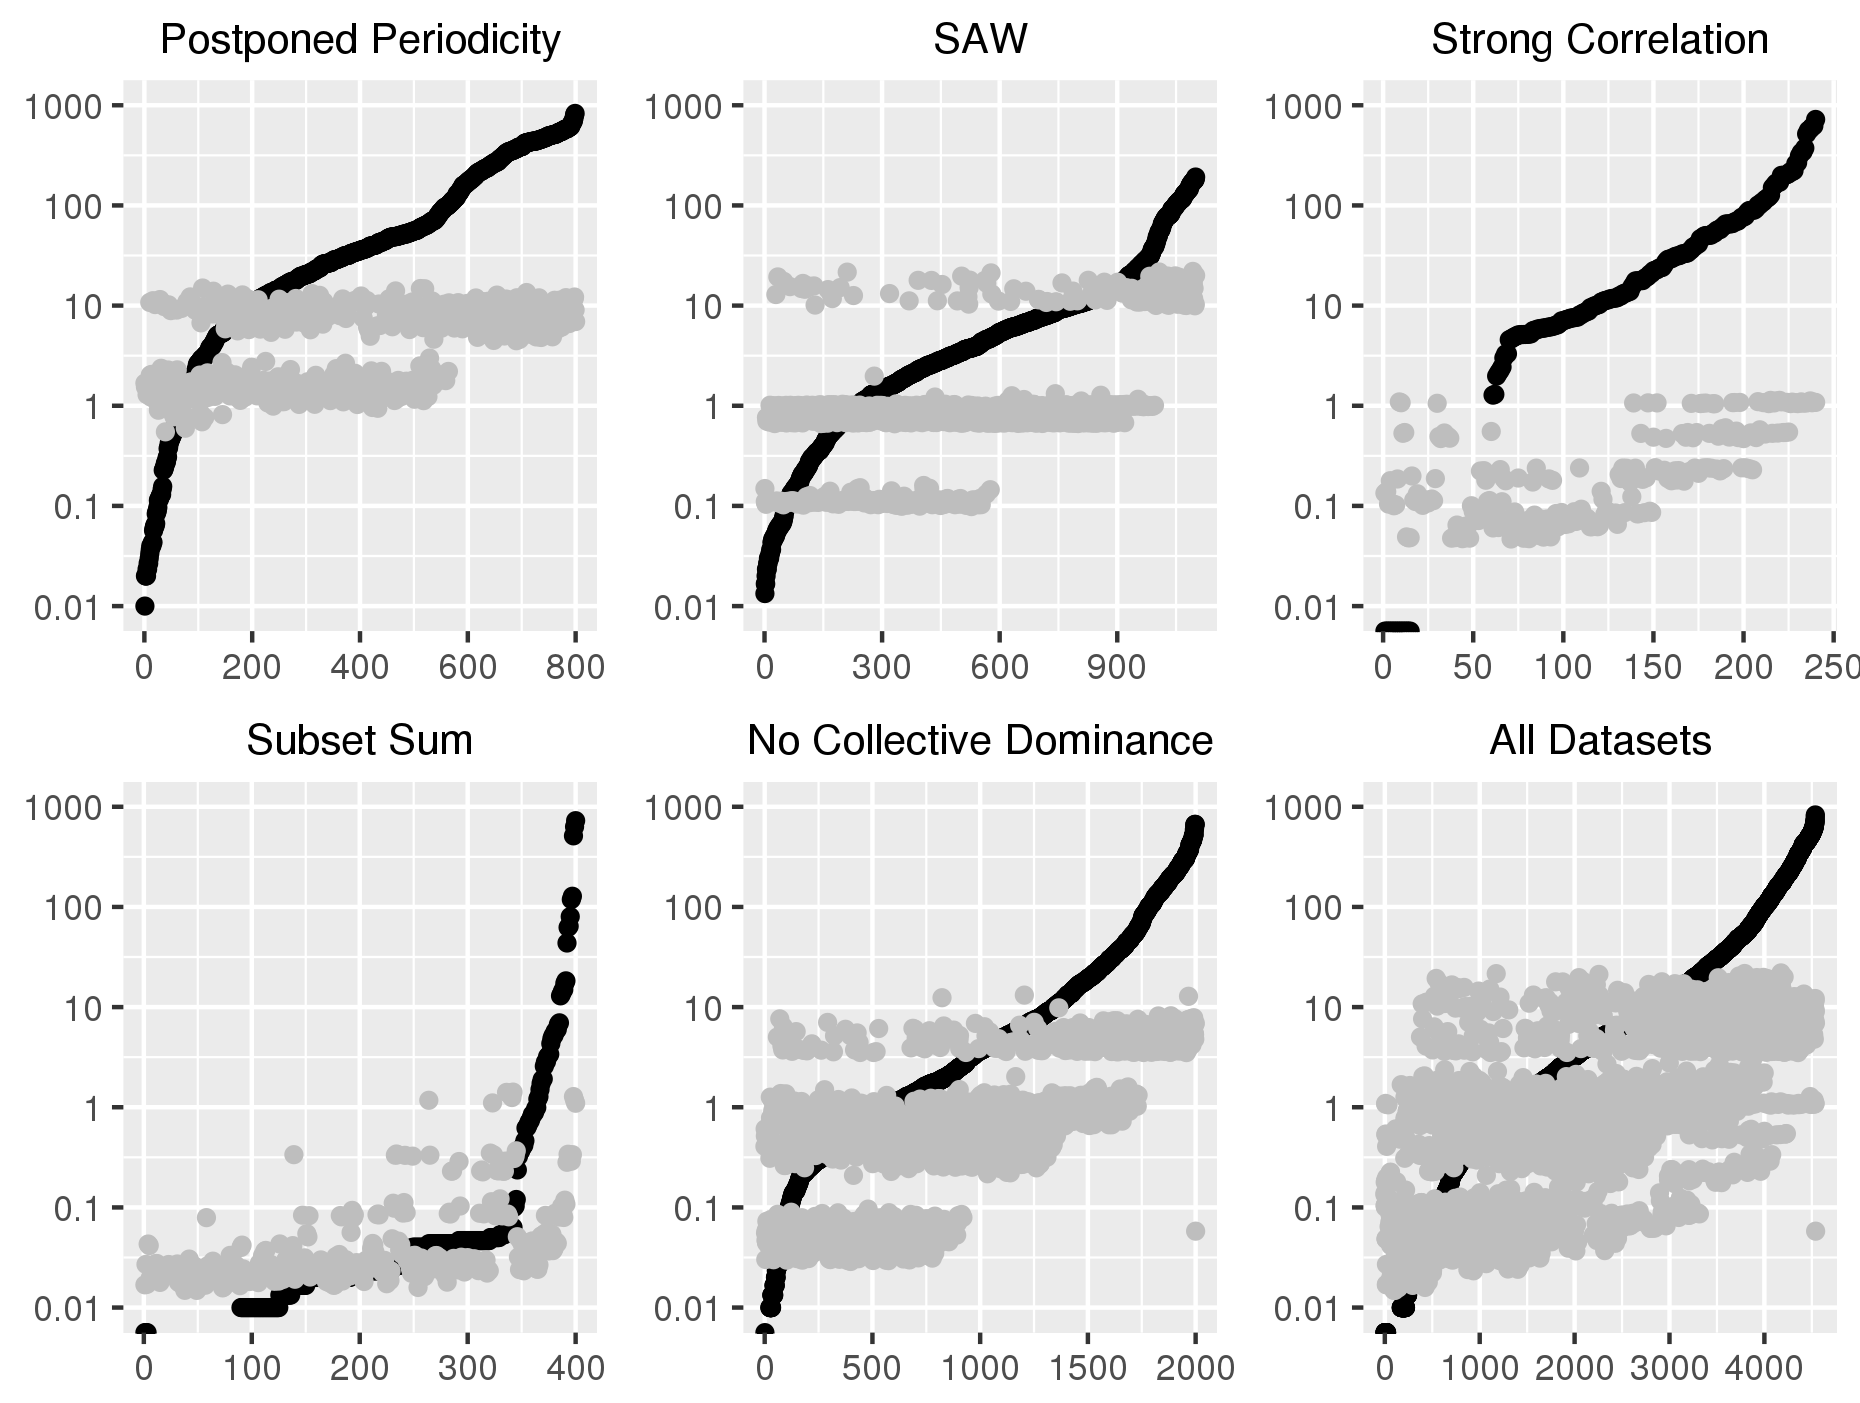
\includegraphics[width=\textwidth]{six_plots.png}
  \caption{The times used by UKP5 and PYAsUKP for each instance of each class. The black dots represent PYAsUKP times. The gray dots represent UKP5 times. The y axis is time used to solve an UKP instance, in seconds. The x axis is the instance index when the times are sorted by increasing PYAsUKP time. \textbf{Note that the y axis is in logarithmic scale.}}
\end{figure}

For the instances that are solved by B\&B in short time, the DP is not competitive against B\&B. 
The UKP5 can't compete with PYAsUKP on easy datasets, as only the time for initializing an array of size \(c\) is already greater than the B\&B time. 
Nonetheless, for hard instances of combinatorial problems, B\&B is known to show a bad worst case performance (exponential time). 
As EDUK2 combines B\&B and DP with the intent of getting the strengths of both, and none of its weaknesses, we found anomalous that this typical B\&B behavior was present in PYAsUKP. 
We executed PYAsUKP with the \emph{-nobb} flag, that disables the use of B\&B. 
The PYAsUKP with disabled B\&B had a performance worst than the one with B\&B. 
For the presented classes, the ratios $\frac{\textit{no-B\&B~avg~time}}{\textit{B\&B~avg~time}}$ by instance class are: 
Subset-sum: 5.70; Strong correlation: 2.47; Postponed periodicity: 2.61; No collective dominance: 4.58; SAW: 4.07. 
For almost every individual instance no-B\&B was worse than B\&B (and when no-B\&B was better this was by a small relative difference). 
Based on this evidence, we conclude that the PYAsUKP implementation of the EDUK2 DP-phase is responsible for the larger maximal PYAsUKP times (the time seems exponential but it is instead pseudo-polynomial with a big constant).

%Based on the first statement, and the discovery that the EDUK2 DP phase was responsible for the 
Looking back at the first statement of this section, we can now conclude that for instances that are hard for B\&B, UKP5 clearly outperforms PYAsUKP DP by a big constant factor. 
Even considering the instances that PYAsUKP solves almost instantly (because of B\&B), UKP5 is about 47 times faster than PYAsUKP, in average. 
If we ignored the advantage given by B\&B (giving UKP5 a B\&B phase, or removing the one used on EDUK2) this gap would be even greater.

We also compared our results with CPLEX.
In~\cite{pya} the authors presented results for CPLEX version 10.5, and showed that EDUK2 outperformed CPLEX.
However, CPLEX efficiency has grown a lot in the last versions. Due to this, we run CPLEX 12.5.
For the instances tested, UKP5 outperformed CPLEX 12.5 considerable.
For the presented classes, the ratios $\frac{CPLEX~avg~time}{UKP5~avg~time}$ by instance class are: 
Subset-sum: 258.11; Strong correlation: 64.14; Postponed periodicity: 12.18; No collective dominance: 16.23; SAW: 120.14. 
Moreover, we set a time limit of 1,000 seconds and a memory limit of 2GB for CPLEX, while every UKP5 and PYAsUKP run finished before these limits.
The ratios above were computed considering 1,000 seconds for the instances that reached the time limit.
However, from 4540 instances, in 402 runs the CPLEX reached the time limit.
In 8 instances CPLEX reached the memory limit. 
We did not compare UKP5 with MTU2 since PYAsUKP already outperformed it, as shown in~\cite{pya}.
However, in a future work we intend to reimplement MTU2 to allow the comparison on the hard instances where it presented overflow problems.

The average UKP5 implementation memory consumption was greater than the PYAsUKP memory consumption. For each instance class, the UKP5-to-PYAsUKP memory consumption ratio was: Subset-sum: \(10.09\); Strong correlation: \(2.84\); Postponed periodicity: \(1.62\); No collective dominance: \(12.41\); SAW: \(1.31\). 
However, note that the UKP5 memory consumption worst case is \(n + 2\times c\) (pseudo-polynomial on \(n\) and \(c\)). 
The UKP5 consumed at most \(\approx 1.6\)G solving an instance.

\section{Conclusion and Final Remarks}

In this work we present UKP5, a new algorithm to solve the Unbounded Knapsack Problem based on dynamic programming.
UKP5 outperformed PYAsUKP, the only known implementation of EDUK2, the state-of-the-art algorithm for solving the problem.
We computed the speedups calculated as the ratio of times between the two algorithms, and UKP5 is two orders of magnitude faster on average, considering the 4540 tested instances.

The core idea of UKP5 is to apply five improvements over a previously proposed dynamic programming algorithm.
An analysis on the individual performance impact caused by each one of the five UKP5 improvements (see Section \ref{sec:ukp5}) will be presented in an extended version of this paper. 
Future works on the UKP5 should consider the following unanswered questions: Can arrays slices or a heap be used to reduce UKP5 memory consumption without a big performance loss? 
Combined with our periodicity check, the change in the data structure could improve UKP5 performance on instances where only a fraction of \(c\) is iterated? 
PYAsUKP shows that the addition of a B\&B phase before the DP can give good results, how could we apply the same idea to UKP5 and how would be the results?
How is the performance of UKP5 applied in real-world instances generated by the column generation iterations for BPP and CSP?

\subsection{Acknowledgments}

We are very thankful to Vincent Poirriez for providing us the codes of a stable version of PYAsUKP, and answering our doubts about the paper~\cite{pya}. 
We are thankful to the CNPq (Conselho Nacional de Desenvolvimento Cient\'ifico e Tecnol\'ogico) for the financial support.
% the master's degree scholarship of Henrique Becker, without its financial support this research would not be possible.

%\section{Appendix}
\begin{comment}
\begin{table}
\caption{Columns \textbf{n} and \(w_{min}\) values must be multiplied by \(10^3\) to obtain their true value. Let \(T\) be the maximal memory used by UKP5 or EDUK2 as reported by the \emph{time} tool, then the meaning of the columns \textbf{avg}, \textbf{sd}, \textbf{min} and \textbf{max}, is, respectively, the arithmetic mean of \(T\), the standard deviation of \(T\), the minimal value of \(T\) and the maximal value of \(T\). The time unit of the table values is Mb (megabytes, not mibibytes).}
\def\arraystretch{1.1}
\setlength\tabcolsep{4px}

\begin{tabular}{@{\extracolsep{4pt}}rrrrrrrrrrr@{}}

\hline
\multicolumn{3}{l}{Instance desc.} & \multicolumn{4}{l}{UKP5} & \multicolumn{4}{l}{PYAsUKP}\\
\cline{1-3}\cline{4-7}\cline{8-11}

\multicolumn{3}{l}{400 inst. per line} & \multicolumn{8}{l}{Subset-sum. Random \emph{c} between \([5\times10^6; 10^7]\)}\\
\cline{1-3}\cline{4-11}

& \textbf{n} & \(w_{min}\)  & \textbf{avg} & \textbf{sd} & \textbf{min} & \textbf{max} & \textbf{avg} & \textbf{sd} & \textbf{min} & \textbf{max}\\
\cline{1-3}\cline{4-7}\cline{8-11}

\multicolumn{3}{c}{See section~\ref{sec:subsetsum}} & 133.96 & 22.85 & 89.85 & 175.67 & 13.28 & 6.71 & 6.28 & 53.28\\

\hline

\multicolumn{3}{l}{20 inst. per line} & \multicolumn{8}{l}{Strong correlation. Random \emph{c} between \([20\overline{n}; 100\overline{n}]\)}\\
\cline{1-3}\cline{4-11}
\textbf{\(\alpha\)} & \textbf{n} & \(w_{min}\) & \textbf{avg} & \textbf{sd} & \textbf{min} & \textbf{max} & \textbf{avg} & \textbf{sd} & \textbf{min} & \textbf{max}\\
\cline{1-3}\cline{4-7}\cline{8-11}
 5 & 5  & 10 & 12.82 & 3.78 & 7.30 & 18.59 & 9.01 & 3.24 & 5.81 & 12.51\\
   &    & 15 & 12.38 & 3.42 & 7.70 & 19.40 & 12.93 & 2.68 & 5.86 & 14.99\\
   &    & 50 & 13.61 & 3.30 & 7.91 & 18.26 & 20.01 & 6.66 & 7.60 & 30.62\\
 5 & 10 & 10 & 105.57 & 36.90 & 36.13 & 153.65 & 7.13 & 0.82 & 6.25 & 8.40\\
   &    & 50 & 106.10 & 39.68 & 36.54 & 159.28 & 21.05 & 10.53 & 6.28 & 33.97\\
   &    & 110 & 103.18 & 34.99 & 37.68 & 149.38 & 41.56 & 22.93 & 6.35 & 78.19\\
-5 & 5  & 10 & 13.06 & 4.27 & 6.88 & 18.99 & 12.81 & 3.67 & 5.85 & 16.23\\
   &    & 15 & 13.81 & 3.43 & 8.56 & 19.30 & 14.33 & 3.81 & 5.85 & 17.92\\
   &    & 50 & 14.61 & 3.22 & 8.33 & 18.76 & 23.17 & 10.39 & 5.86 & 42.08\\
-5 & 10 & 10 & 109.12 & 36.36 & 37.02 & 159.60 & 13.91 & 4.37 & 6.28 & 18.51\\
   &    & 50 & 115.43 & 38.81 & 36.23 & 160.05 & 26.97 & 13.64 & 6.35 & 45.19\\
   &    & 110& 97.20 & 33.97 & 39.73 & 151.94 & 49.22 & 29.02 & 7.94 & 98.78\\
\hline

\multicolumn{3}{l}{200 inst. per line} & \multicolumn{8}{l}{Postponed periodicity. Random \emph{c} between \([w_{max}; 2\times10^6]\)}\\
\cline{1-3}\cline{4-11}
& \textbf{n} & \(w_{min}\) & \textbf{avg} & \textbf{sd} & \textbf{min} & \textbf{max} & \textbf{avg} & \textbf{sd} & \textbf{min} & \textbf{max}\\
%42.80 & 3.98 & 35.65 & 50.54 & 16.12 & 4.70 & 7.84 & 25.20\\
\cline{1-3}\cline{4-7}\cline{8-11}
& 20 & 20 & 42.80 & 3.98 & 35.65 & 50.54 & 16.12 & 4.70 & 7.84 & 25.20\\
& 50 & 20 & 44.76 & 4.12 & 36.82 & 51.72 & 33.60 & 14.51 & 12.12 & 65.98\\
& 20 & 50 & 42.28 & 4.53 & 34.92 & 50.24 & 18.37 & 4.88 & 8.04 & 29.83\\
& 50 & 50 & 44.34 & 4.48 & 36.67 & 51.39 & 39.05 & 13.15 & 14.45 & 63.64\\

\hline

\multicolumn{3}{l}{500 inst. per line} & \multicolumn{8}{l}{No collective dominance. Random \emph{c} between \([w_{max}; 1000\overline{n}]\)}\\
\cline{1-3}\cline{4-11}
& \textbf{n} & \(w_{min}\) & \textbf{avg} & \textbf{sd} & \textbf{min} & \textbf{max} & \textbf{avg} & \textbf{sd} & \textbf{min} & \textbf{max}\\
\cline{1-3}\cline{4-7}\cline{8-11}
&  5 & n & 83.39 & 44.10 & 7.54 & 161.35 & 12.44 & 5.00 & 5.91 & 36.65\\
& 10 & n & 826.66 & 440.19 & 35.86 & 1580.66 & 23.54 & 16.45 & 7.84 & 136.56\\
& 20 & n & 810.90 & 433.39 & 37.86 & 1578.22 & 46.89 & 34.39 & 8.24 & 205.98\\
& 50 & n & 798.77 & 451.91 & 40.37 & 1582.24 & 120.17 & 87.97 & 13.19 & 569.85\\

\hline

\multicolumn{3}{l}{\emph{qtd} inst. per line} & \multicolumn{8}{l}{SAW. Random \emph{c} between \([w_{max}; 10\overline{n}]\)}\\
\cline{1-3}\cline{4-11}
\textbf{qtd} & \textbf{n} & \(w_{min}\) & \textbf{avg} & \textbf{sd} & \textbf{min} & \textbf{max} & \textbf{avg} & \textbf{sd} & \textbf{min} & \textbf{max}\\
\cline{1-3}\cline{4-7}\cline{8-11}
~200 &  10 & 10 & 14.02 & 4.08 & 6.93 & 20.79 & 14.58 & 4.41 & 6.68 & 23.58\\
~500 &  50 &  5 & 15.89 & 3.92 & 8.72 & 23.16 & 17.39 & 3.55 & 11.96 & 27.54\\
~200 &  50 & 10 & 15.99 & 3.98 & 8.62 & 22.86 & 18.72 & 4.05 & 12.26 & 29.46\\
~200 & 100 & 10 & 111.93 & 42.44 & 39.58 & 179.31 & 60.98 & 33.91 & 20.85 & 140.52\\
\hline

\end{tabular}
\end{table}
\end{comment}

\bibliographystyle{splncs03.bst}
\bibliography{ukp5.bib}

\end{document}
